\chapter{関連研究}
\label{chap:relevant}

本章では、情報ダッシュボードに関する研究と
沢山の人がいる状況での計算機を用いたコミュニケーションの支援に関する研究を紹介する。

\newpage

\section{情報ダッシュボード}
\label{chap:dashboard}

情報ダッシュボードのデザイン\cite{few}に関する研究は多くないが,
表示するべき情報を選択する手法\cite{Jones:2015:ECI:2800835.2800963}や,
セルの自動配置手法\cite{Hertzog:2015:BSP:2678025.2701383}などの
研究が存在する.

\subsection{Exist.io}
Jonesはデータ集約ツールに多面的な相関情報を提供することで生じる固有の課題について説明し、
情報ダッシュボードに表示すべき情報を選択する手法をを提案している。
また、その手法で実装されたデータ視覚化システム「Exist.io\footnote{https://exist.io}」(図\ref{existio})を紹介し、
既存のツールを改善するための設計上の考慮事項について述べている。

\begin{figure}[H]
\centering
\fbox{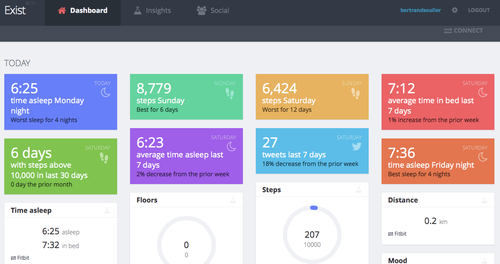
\includegraphics[width=9cm]{images/existio.png}}
\caption{Exist.io}
\label{existio}
\end{figure}

\subsection{Binary Space Partitioning Layouts}
Hertzogは情報ダッシュボードのレイアウトが柔軟性に欠けていることを指摘している\cite{Hertzog:2015:BSP:2678025.2701383}。
今日の多くの情報ダッシュボードアプリケーションはレイアウトのカスタマイズを提供しないか、
レイアウトマネージャを提供していたとしてもしてもその制御が非常に難しい。
そこで、バイナリ空間パーティショニング(Binary Space Partitioning)に基づいた自動レイアウト手法を提案し、
ユーザーが決めたレイアウトを尊重しながら、すべてのタイルの位置とサイズを実際に望ましいサイズに
できるだけ近くなるように計算するアルゴリズムを紹介している(図\ref{hertzog})。


\begin{figure}[H]
\centering
\fbox{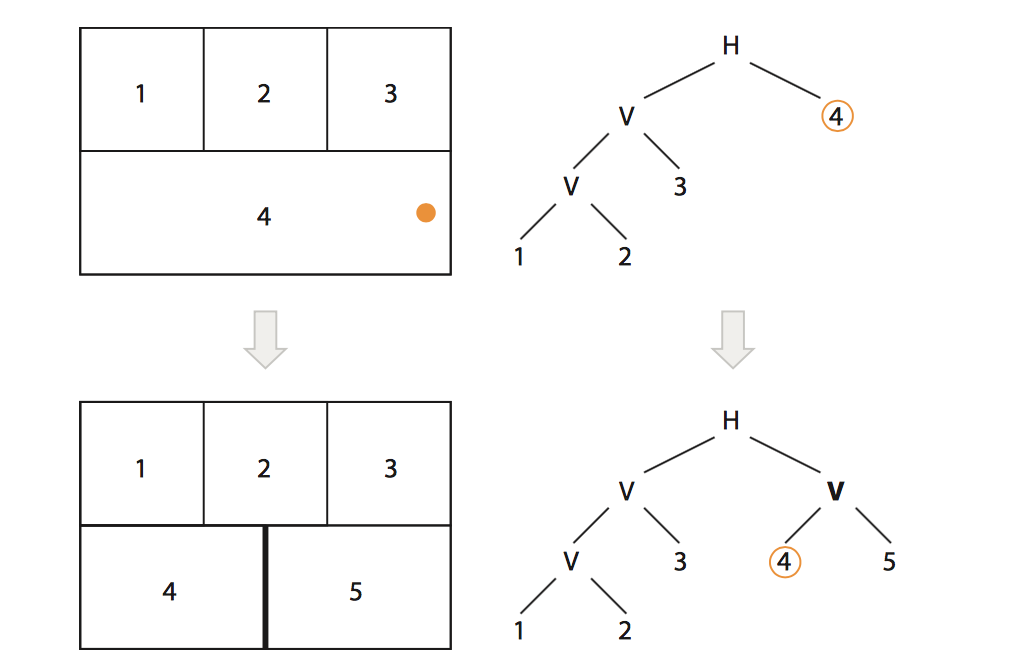
\includegraphics[width=9cm]{images/hertzog.png}}
\caption{バイナリ空間パーティショニング}
\label{hertzog}
\end{figure}


\section{沢山の人がいる状況での計算機を用いたコミュニケーションの支援}

\subsection{Lock-on-Chat}

西田らによる「Lock-on-Chat\cite{nishida2006}」(図\ref{lockonchat})は複数の話題に分散した会話を促進するチャットシステムである。
Lock-on-Chatは参加者間で画像を共有し、
それらの画像の特定部分に会話を結びつける機能が特徴である。
文書や画像と会話を結びつけるほかのシステムが,ひとつの対象について深く議論するのに適しているのに対して,
は複数の画像に分散した会話をしやすくすることに重きを置いてデザインされている.
Lock-on-Chatは学術会議 (WISS2004, 2005) において発表中に聴衆が会話するためのシステムとして運用された。

\begin{figure}[H]
\centering
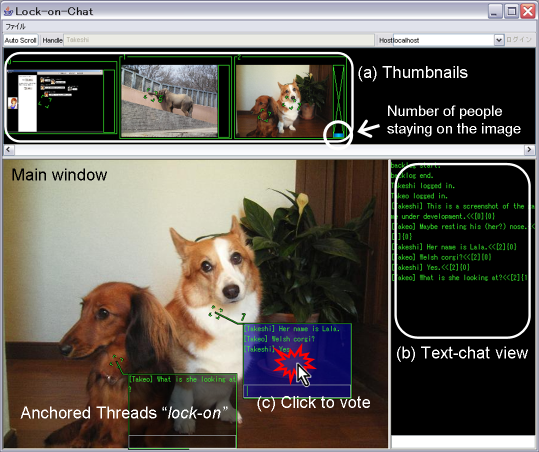
\includegraphics[width=8cm]{images/lockonchat.png}
\caption{Lock-on-Chat}
\label{lockonchat}
\end{figure}


\subsection{On-Air Forum}

西田らによる「On-Air Forum\cite{nishida2011}」(図\ref{onairforum})は
コンテンツへの没頭度合いに応じた発言の入力方法を提供するチャットシステムである。
従来のチャットシステムでは、
コンテンツとコミュニケーションを同時並行的に把握し続けるのは参加者にとっての負荷が高く,
コンテンツを視聴中の興奮やほかの発言に対する同意といった単純な反応を返すことで精いっぱいになってしまう
ことを問題としており、
コンテンツに没頭しているときでも利用できるエキサイトメッセージ機能,
テキストを入力する余裕がないときでも利用できる反応ボタンと選択肢付き発言機能を提供している。

\begin{figure}[H]
\centering
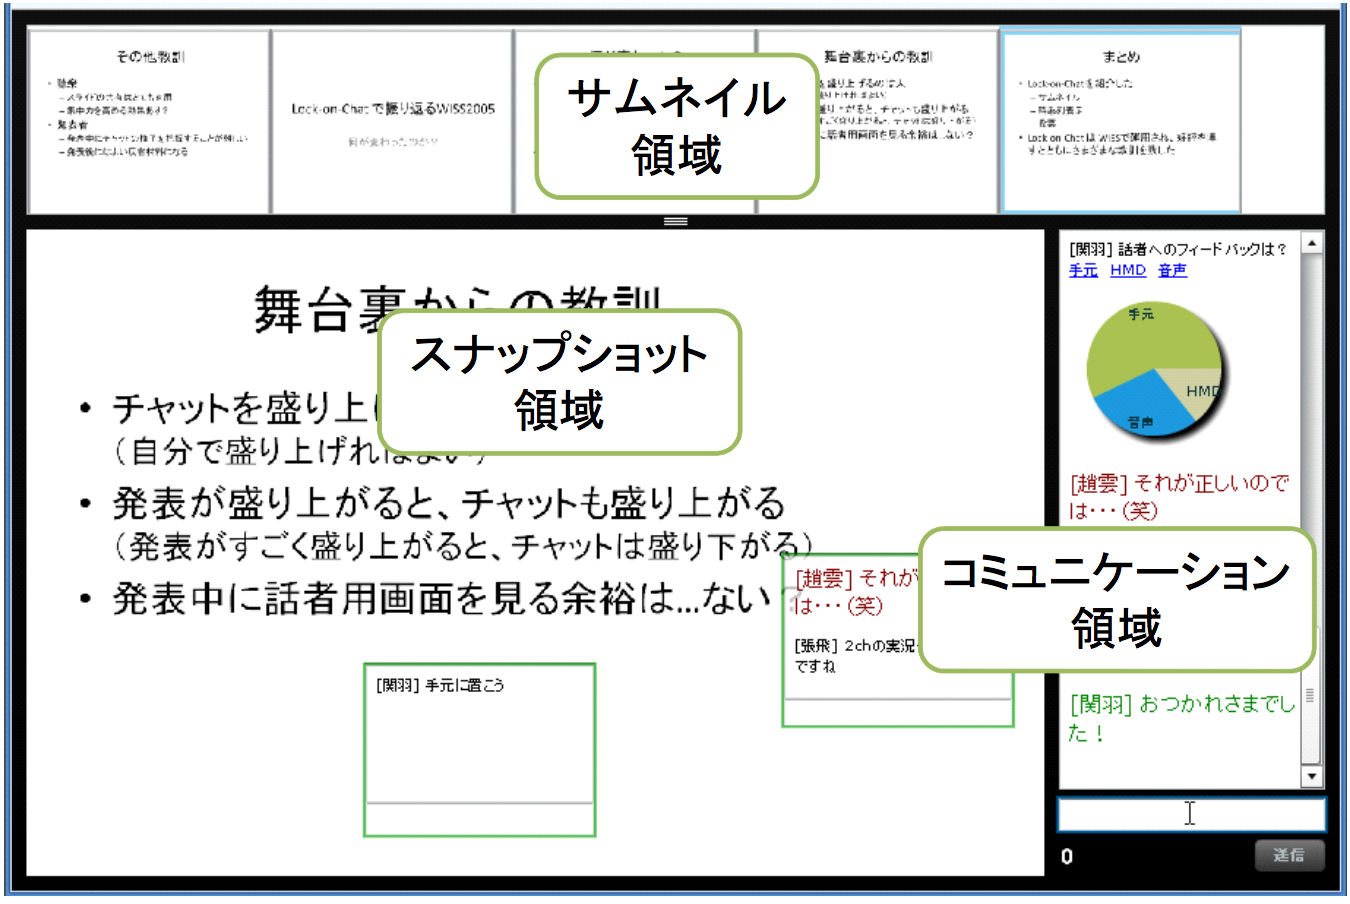
\includegraphics[width=8cm]{images/onairforum.png}
\caption{On-Air Forum}
\label{onairforum}
\end{figure}

\subsection{二次元チャットシステム}

二次元チャットシステム(図\ref{2dchat})とは、二次元情報を持つキャンバス上で
自由な位置に発言をオブジェクトとして配置することでチャットを行うシステムである。
発言を視覚的にグループ分けできるため、複数の話題に対し同時に会話を行うことができる。
また、キャンバスへの書き込み機能や画像の挿入機能などを備えたシステム\cite{kazama}や
実空間の会話の音声とチャットのやりとりを関連付けることのできるシステム\cite{110002711453}を利用することで、
タイムライン形式のチャットシステムよりもインタラクティブなチャットを行うことができる。
しかし、二次元チャットシステムは多人数が複数の場所で会話を行っているため、
全ての発言を把握することが困難である。
また、時間軸が存在しないため、会話の流れを把握しにくいという問題がある。

\begin{figure}[H]
\centering
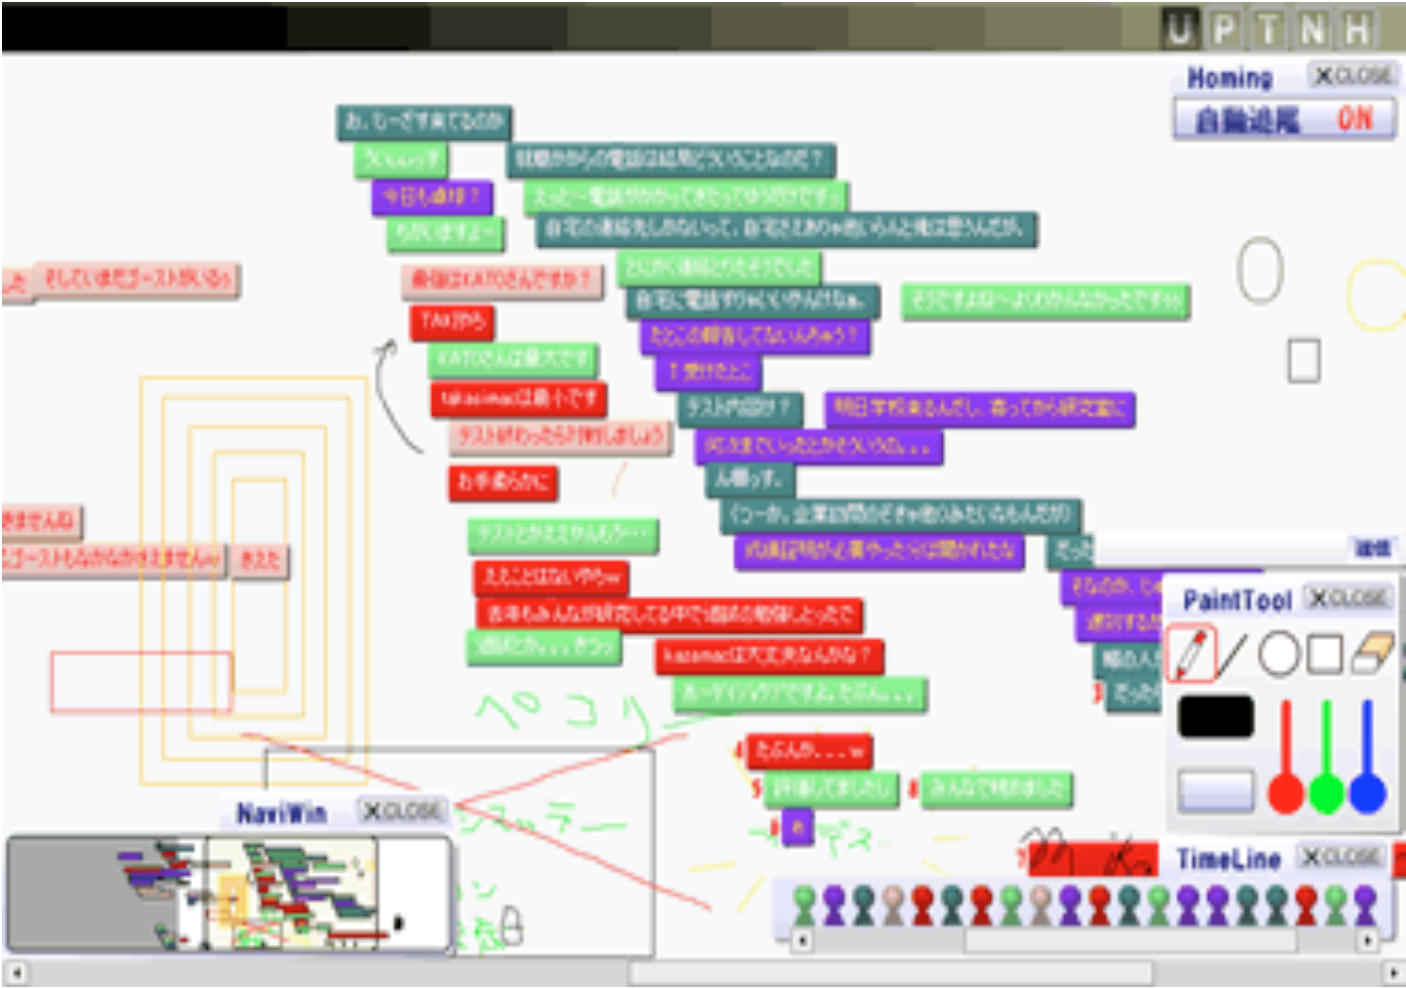
\includegraphics[width=8cm]{images/2dchat.png}
\caption{二次元チャットシステム「firefly」}
\label{2dchat}
\end{figure}


\subsection{ラジへぇ}

加藤らの「ラジへぇ\cite{110009657336}」(図\ref{rajihe})はラジオ聴取時における感想共有システムである。
加藤らは、ラジオの「別の作業をしながらでも聴ける」という聴取スタイルに着目し,
効果音をリアルタイムに鳴らし合うことでラジオ番組に対する感想を共有するシステムを提案している。
あらかじめ用意された単純な感想をボタンを押して選択することで感想の共有を簡単にし、
音声によるフィードバックで画面を目で追えない状況でも他人の感想を知れるような工夫がなされている。

\begin{figure}[H]
\centering
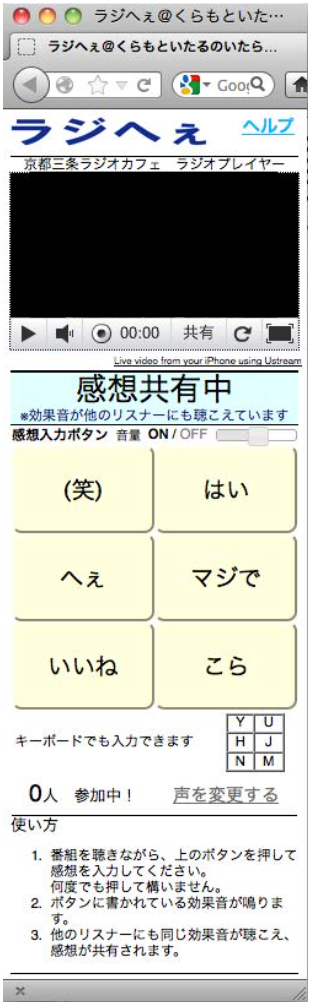
\includegraphics[width=3cm]{images/rajihe.png}
\caption{ラジへぇ}
\label{rajihe}
\end{figure}


\subsection{World Cupinion}

Shiraziらはスマートフォン上の非言語的なアイコンを用いたUIを通して
テレビ番組に関するリアルタイム意見共有システム「World Cupinion」を
提案している\cite{SahamiShirazi:2011:RNO:1978942.1978985}。
感想の投稿のインタフェースは「ラジへぇ」と同じように
あらかじめ用意された単純な感想をアイコンで表したボタンを押すことで
感想の投稿をするものであるが、
一人ひとりの感想を共有するのではなく
それぞれの感想を持った人の割合を表示している。
Shiraziらは、FIFAワールドカップ2010\footnote{http://www.fifa.com/worldcup/archive/southafrica2010/}開催時に
「World Cupinion」のアプリケーションを配布して非公式な実証実験を行っており、
後から放送された番組を見返したときに、集約された感想がテレビ番組の要約に役立ったと述べている。


\begin{figure}[H]
\centering
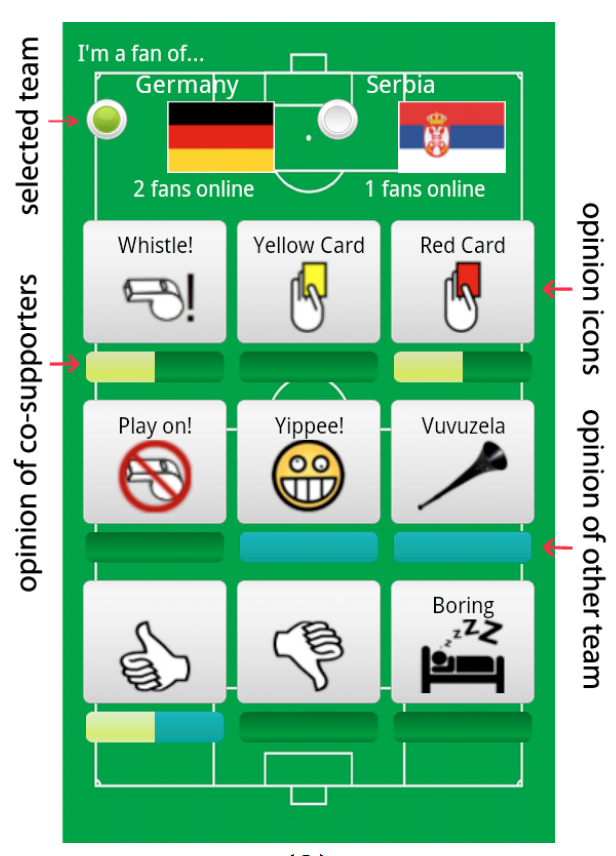
\includegraphics[width=5cm]{images/worldcupinion.png}
\caption{World Cupinion}
\label{worldcupinion}
\end{figure}


\subsection{SIGSHY}

近年,
消極的な人間でも会議の議論などに参加しやすくするための研究が
消極性研究会(SIGSHY: Special Interest Group on Shyness and Hesitation around You)
というグループなどを中心に盛んになってきているが\cite{kurihara2016}\cite{nishida2011},
本論文で提案するシステムもこのような方向性の支援に利用できると考える.